\documentclass{standalone}

\usepackage{graphicx}
\usepackage{caption}
\usepackage{tikz}
\usetikzlibrary{positioning,shapes.symbols,matrix,arrows}

\begin{document}

% \begin{tikzpicture}
%     [%%%%%%%%%%%%%%%%%%%%%%%%%%%%%%
%     box/.style={rectangle,draw=black,thick, minimum size=1cm},
%     ]%%%%%%%%%%%%%%%%%%%%%%%%%%%%%%

%     \draw[step=1cm,color=gray] (0,0) grid (10,10);


%     % agent
%     \node[box,fill=red] at (4.5,4.5)(agent){};
%     \node at (5,2.5) (agent_text) {agent};
%     \draw [-stealth](agent_text) -- (agent);

%     % goal
%     \node[box,fill=green] at (8.5,2.5)(goal){};
%     \node at (7,1.5) (goal_text) {goal};
%     \draw [-stealth](goal_text) -- (goal);
%     \node[box,fill=green] at (2.5,+3.5) {};
%     \node[box,fill=green] at (5.5,+7.5) {};
%     \node[box,fill=green] at (2.5,+6.5) {};
%     \node[box,fill=green] at (7.5,+8.5) {};

%     % norm
%     \draw[very thick][orange] (2,5) -- (2,9);
%     \node at (3.5,8.8) (norm_text) {norm};
%     \draw [-stealth](norm_text) -- (2.5,8);
%     \draw[very thick][orange] (2,8) -- (4,8);
%     \draw[very thick][orange] (4,7) -- (5,7);
%     \draw[very thick][orange] (7,5) -- (9,5);
%     \draw[very thick][orange] (3,5) -- (3,4);
%     \draw[very thick][orange] (4,4) -- (4,3);
%     \draw[very thick][orange] (3,3) -- (3,2);
% \end{tikzpicture}

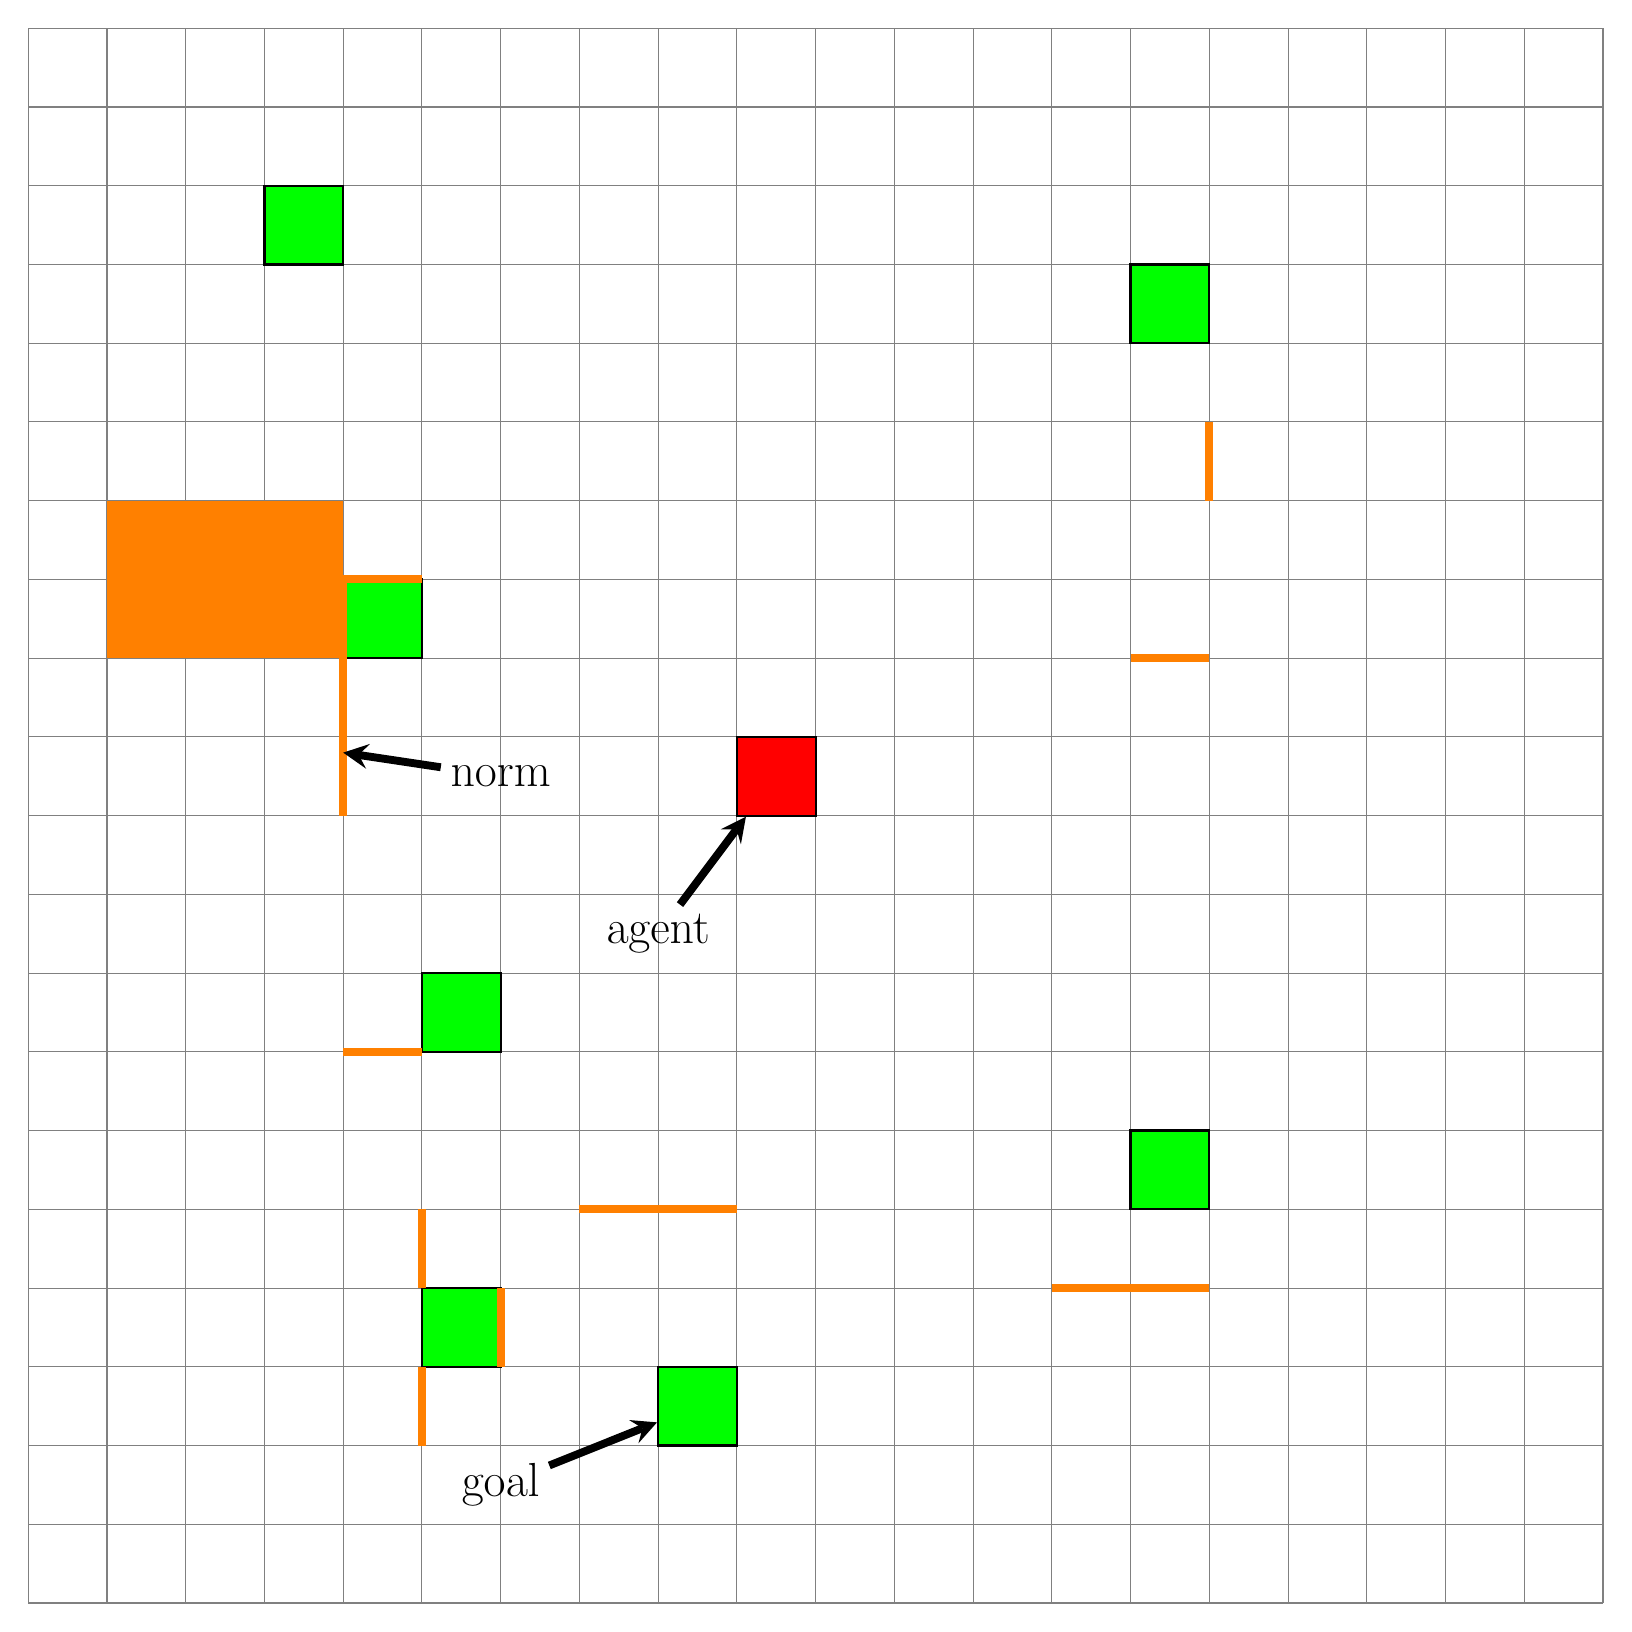
\begin{tikzpicture}
    [%%%%%%%%%%%%%%%%%%%%%%%%%%%%%%
    box/.style={rectangle,draw=black,thick, minimum size=1cm},
    ]%%%%%%%%%%%%%%%%%%%%%%%%%%%%%%

    \draw[step=1cm,color=gray] (0,0) grid (20,20);


    % agent
    \node[box,fill=red] at (9.5,10.5)(agent){};
    \node at (8,8.5) (agent_text) {\LARGE{agent}};
    \draw [-stealth,line width=0.1cm](agent_text) -- (agent);

    % goal
    \node[box,fill=green] at (8.5,2.5)(goal){};
    \node at (6,1.5) (goal_text) {\LARGE{goal}};
    \draw [-stealth,line width=0.1cm](goal_text) -- (goal);
    \node[box,fill=green] at (5.5,3.5) {};
    \node[box,fill=green] at (5.5,+7.5) {};
    \node[box,fill=green] at (4.5,+12.5) {};
    \node[box,fill=green] at (14.5,+16.5) {};
    \node[box,fill=green] at (14.5,+5.5) {};
    \node[box,fill=green] at (3.5,+17.5) {};

    % norm
    \draw[line width=0.1cm][orange] (4,10) -- (4,13);
    \node at (6,10.5) (norm_text) {\LARGE{norm}};
    \draw [-stealth, line width=0.1cm](norm_text) -- (4,10.8);

    \draw[line width=2cm][orange] (1,13) -- (4,13);

    \draw[line width=0.1cm][orange] (3,13) -- (5,13);
    \draw[line width=0.1cm][orange] (4,7) -- (5,7);
    \draw[line width=0.1cm][orange] (7,5) -- (9,5);
    \draw[line width=0.1cm][orange] (5,5) -- (5,4);
    \draw[line width=0.1cm][orange] (6,4) -- (6,3);
    \draw[line width=0.1cm][orange] (5,3) -- (5,2);
    \draw[line width=0.1cm][orange] (15,14) -- (15,15);
    \draw[line width=0.1cm][orange] (14,12) -- (15,12);
    \draw[line width=0.1cm][orange] (13,4) -- (15,4);
\end{tikzpicture}
\end{document}